\chapter{Step 0: Foundation} \label{dev-step0}

\begin{abstract}
    Part 2 of this dissertation defines specific implementations of each method considered: MORDM, multi-scenario MORDM, and MORO. It also specifies the value ranges of uncertainties and levers, practical definitions of the outcomes of interest, and the functional structure of each problem variation: intertemporal, DPS, and planned adaptive DPS. 
    
    This first chapter provides a background on how the implementations of both methods and problem variations were developed, and will describe the specific definition of robustness used across this analysis, which will be referenced in more than one step of the analysis.
\end{abstract}

\begin{figure}[h]
    \centering
    \captionsetup{justification=centering}
    
    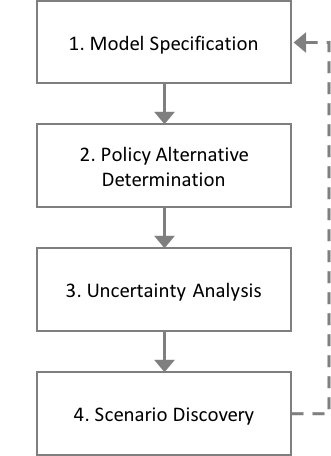
\includegraphics{structure-step0}
    \caption{Basic RDM analysis structure}
    \label{fig:structure-step0}
\end{figure}

\newpage

\section{Implementation Structure}
The implementation structure will follow the fundamental flow of the RDM process, with each of the next four chapters describing a step of an RDM-based decision support process, found in \cref{fig:structure-step0}. \cref{dev-step1} contains the model specification for all three variations of the lake problem. \cref{dev-step2} defines the policy alternative determination process for each of the three methods. As this step is where the key methodological difference lies, \cref{dev-step2} contains critical information that differentiates each method. Next, \cref{dev-step3} describes the process of uncertainty analysis, including the method of determining how robust each policy alternative is considered. The final step in the RDM process is scenario discovery, which is discussed in \cref{dev-step4}. Finally, this part concludes by establishing the points of comparison that will be considered in \cref{dev-comparisons}.

\section{Definition of Robustness}\label{step0-robust}
The review in \cref{review-robustness} described several options for determining robustness of policies under conditions of deep uncertainty. Traditionally, the desired robustness metric specification is determined through conversations between analysts and decision makers to ensure that goals of decision makers are being met. Often, the involved parties will consider multiple robustness metrics for the same analysis to provide a broader picture of the robustness of each policy \citep{Quinn2017}. 

To facilitate the comparison of results across methods in this study, a single common definition for robustness will be used: the domain criterion measure. The domain criterion measure, a satisficing metric, will provide the most effective and straightforward way to focus on policies that ensure minimum thresholds of performance are met when considering conflicting objectives. This metric is suitable wherever robustness is used in all three methods of analysis under consideration. 

As a reminder, domain criterion satisficing is defined as the fraction of all considered future states of the world (SOWs) in which a threshold of performance is met \citep{Starr1963}. This results in a metric value between 0 and 1, where 0 indicates that no set of uncertainty values produced an outcome that met the defined threshold given a specific policy configuration, and 1 indicates perfect performance. The threshold values and goal for each outcome can be found in \cref{table:robust-thresholds}. 

\begin{table}[h]
    \centering
    \captionsetup{width=0.55\textwidth}
    \caption{Robust threshold values for each outcome of interest of the lake problem}
    \label{table:robust-thresholds}
    
    \setlength\arrayrulewidth{1pt}\arrayrulecolor{white}
    \rowcolors{2}{odd-row-blue}{even-row-blue}
    \begin{tabularx}{0.55\textwidth}{l|l|l}
        \rowcolor{tudelft-dark-blue!80}
        \color{white}\bfseries Outcome  &  \color{white}\bfseries Goal  &  \color{white}\bfseries Threshold  \\ 
        \hline
        Pollution Level   & Minimize      & Critical Pollution Level            \\ \hline
        Utility           & Maximize      & \multicolumn{1}{|r|}{0.75}          \\ \hline
        Inertia           & Maximize      & \multicolumn{1}{|r|}{0.99}          \\ \hline
        Reliability       & Maximize      & \multicolumn{1}{|r|}{0.8}           \\
    \end{tabularx}
\end{table}

These values are generally based on previous research that has developed and tested the lake model \citep{Quinn2017, Singh2015}, save the pollution level. One difference relates to the threshold for the pollution level. Previous research has used a static value for the pollution threshold when determining robustness. This study proposes using the critical pollution level as defined by \citet{Quinn2017} as the threshold for the lake's pollution level.

\subsection{Minimizing the maximum pollution level}
The first outcome of interest, indicating the interests of environmental protection groups, is defined as the fraction of SOWs whose maximum level of pollution remains under the critical pollution threshold (the tipping point after which it is impossible to return the lake to al oligotrophic state without manual intervention). The critical pollution threshold is defined in \cref{eq:critp}, where b and q refer to specific values of the uncertainty inputs to the lake model, b and q, and X represents the level of pollution under consideration \citep{Quinn2017}. This function produces two intercepts, the first of which represents the critical pollution threshold, $Pollution_{crit}$. 

During execution, one experiment out of the set of N states of the world (which is a pairing of an SOW and a set of lever values that constitute a policy) generates T releases of pollution into the lake, the maximum value of which is returned. The robustness metric is then calculated by determine the fraction of experiments for which the pollution level remains under the critical P threshold. 

\begin{equation}\label{eq:critp}
    \frac{X^{q}}{(1+X^{q})}-b*X
\end{equation}

\subsection{Maximizing utility}
Also known as expected economic benefits for the town (through industry and agriculture), utility of robustness is determined as the fraction of experiments for which their average utility level is above the threshold defined in \cref{table:robust-thresholds}. The first component of this metric is to determine the utility of a policy in an experiment, known as the discounted economic benefits. This value is determined for every year in the time period of interest. Discounted economic benefit for one year of the simulation run is defined in \cref{eq:utility}, and involves two parameters from the set of uncertain parameters to be discussed in \cref{dev-step1}: $\alpha$ and $\delta$. The vector of expected utility values calculated using \cref{eq:utility} are then averaged to get a single value that is used to calculate robustness. 

\begin{equation}\label{eq:utility}
    \sum_{t=0}^{T-1}\alpha*a_{t}*\delta^{t}
\end{equation}

\subsection{Maximizing inertia}
As discussed in \cref{review-problems} the lake manager has an interest in maintaining as stead a release rate of pollution as possible, to avoid unnecessary expenses that occur from rapid changes in release levels. Therefore, the third robust outcome of interest is to maximize the average inertia of a policy. Like utility, inertia of an policy and for an experiment is first calculated for every time step involved. The mean of that vector of values is what is used to determine inertia-based robustness. Inertia for a single time step in an experiment is determined with \cref{eq:inertia}. 

\begin{equation}\label{eq:inertia}
    \sum_{t=1}^{T-1}\phi_{t}, \text{where } \phi_{t} = \begin{cases}
    1 & |X_{t}-X_{t-1}| < 0.01| \\
    0 & \text{otherwise}
    \end{cases}
\end{equation}

\subsection{Maximizing reliability}
The last robust outcome of interest to define is reliability. As reliability indicates the likelihood that a policy will lead to pollution levels remaining under the critical p threshold, the lake manager and other parties interested in keeping the lake healthy are seeking policies in which a high fraction of policies yield potential futures in which the pollution level stays consistently below the critical pollution level, and so it is another maximizing objective. The reliability of a single experiment is determined as the average of the reliability measures for each time step, shown as \cref{eq:reliability} \citep{Ward2015}.

\begin{equation}\label{eq:reliability}
\sum_{t=1}^{T}\theta_{t}, \text{where } \theta_{t} = \begin{cases}
1 & X_{t} < P_{crit} | \\
0 & \text{otherwise}
\end{cases}
\end{equation}